% RECOVERED PARTIAL 20260708
% Reconstructed from Codex log sed/nl fragments.
% Gaps below mark original line ranges not present in recovered logs.

% =====================================================================
% Experimental Astronomy (Springer) journal layout -- EMULATED.
% Compile with XeLaTeX (e.g. latexmk -pdfxe).
% Auto-generated from the NIM-A elsarticle source by build_ea_format.py;
% only the journal FORMAT changed -- text, figures, tables, and references
% are carried over verbatim from balloon511_nima_draft_zh.tex.
% For submission, replace this emulated preamble with the official Springer
% Nature class (sn-jnl.cls); the structure is already aligned to it.
% =====================================================================
\documentclass[11pt]{article}
\usepackage[a4paper,top=2.4cm,bottom=2.5cm,left=2.0cm,right=2.0cm]{geometry}
\usepackage{amsmath,amssymb}
\usepackage[UTF8]{ctex}
\usepackage{fontspec}
\setmainfont{TeX Gyre Termes}
\usepackage{booktabs}
\usepackage{graphicx}
\usepackage[section]{placeins}
\graphicspath{{../}}
\renewcommand{\topfraction}{0.92}
\renewcommand{\bottomfraction}{0.8}
\renewcommand{\textfraction}{0.07}
\renewcommand{\floatpagefraction}{0.75}
\usepackage{xcolor}
\usepackage{tikz}
\usetikzlibrary{arrows.meta,positioning}
\usepackage{caption}
\captionsetup{font=small,labelfont=bf}
\usepackage{titlesec}
\titleformat{\section}{\normalfont\large\bfseries}{\thesection}{0.6em}{}
\titleformat{\subsection}{\normalfont\normalsize\bfseries}{\thesubsection}{0.5em}{}
\titlespacing*{\section}{0pt}{1.3ex plus .2ex minus .2ex}{0.6ex}
\titlespacing*{\subsection}{0pt}{1.0ex plus .2ex minus .2ex}{0.5ex}
\usepackage{fancyhdr}
\pagestyle{fancy}
\fancyhf{}
\fancyhead[L]{\small\itshape Experimental Astronomy}
\fancyhead[R]{\small\thepage}
\renewcommand{\headrulewidth}{0.4pt}
\usepackage{hyperref}
\hypersetup{hidelinks}
\setlength{\emergencystretch}{3em}
\newcommand{\keV}{\,\mathrm{keV}}
\newcommand{\MeV}{\,\mathrm{MeV}}
\newcommand{\cms}{\,\mathrm{cm^{-2}\,s^{-1}}}
\newcommand{\phcms}{\,\mathrm{ph\,cm^{-2}\,s^{-1}}}
\newcommand{\cps}{\,\mathrm{s^{-1}}}
\newcommand{\wii}{W_{511}}
\newcommand{\aeff}{A_{\mathrm{eff}}}
\newcommand{\fzero}{F_{0}}
\newcommand{\fthree}{F_{3\sigma}}
\newcommand{\added}[1]{{\color{red}#1}}
\newcommand{\rewritten}[1]{{\color{green!45!black}#1}}
\newenvironment{addedblock}{\begingroup\color{red}}{\endgroup}
\newenvironment{rewrittenblock}{\begingroup\color{green!45!black}}{\endgroup}

\begin{document}
\thispagestyle{fancy}
\begin{flushleft}
{\LARGE\bfseries 气球载 511 keV Laue 透镜 TES 望远镜本底和未分辨线灵敏度的探测器耦合 Monte Carlo 估计 \par}
\vspace{1.1em}
{\large 作者信息暂隐\par}
\vspace{0.3em}
{\normalsize\itshape 单位信息暂隐\par}
\end{flushleft}
\vspace{0.7em}
\noindent\rule{\textwidth}{0.4pt}
\vspace{0.5em}

\noindent\textbf{Abstract}\hspace{0.7em}银河系 511 keV 湮灭辐射主要由延展的核球和银盘成分主导，而任何紧凑或点状贡献的强度仍不确定。指向式聚焦观测可以探测这一互补的观测域，但前提是气球高度上的大气和仪器诱发本底得到良好控制。本文给出一种气球载望远镜的探测器耦合 Monte Carlo 估计，该望远镜由 10 m Ge(111) Laue 透镜与过渡边缘传感器（transition-edge sensor, TES）微量热计焦平面构成。信号链中，Laue 光学先生成单色轴上 511 keV 点源在焦面的聚焦相空间，随后将通过 Be 入射孔径的光子在探测器/低温系统质量模型中重放；本底链中，瞬发大气粒子/光子和延迟活化衰变在同一探测器/低温系统模型中输运，其中延迟衰变以活化计算所记录的放射性核素产生位置为初始点生成。三类探测器层事例随后用同一 $510.79$--$511.21\keV$ 能窗、CsI 反符合 veto 和拓扑/视场一致性选择进行分析。对入射点源流量 $10^{-4}\phcms$，第 15 天的选后信号率和本底率分别为 $1.19\times10^{-3}\cps$ 和 $3.92\times10^{-2}\cps$，瞬发大气事例占选后本底的 93.4\%。在连续在源曝光假设下，将这些率折叠到所采用的合成 20 d 轨迹，得到诊断性计数显著度 $Z_{20\mathrm{d}}=7.80$，以及相应的 $3\sigma$ 流量阈值 $3.85\times10^{-5}\phcms$。该阈值给出参考模型下谱学未分辨 511 keV 点源的飞行灵敏度估计；选后本底由瞬发大气成分主导，为屏蔽、准直和材料选择等设计优化指明了方向。

\vspace{0.7em}
\noindent\textbf{Keywords}\hspace{0.7em}伽马射线仪器 $\cdot$ 511 keV 湮灭线 $\cdot$ 过渡边缘传感器微量热计 $\cdot$ Laue 透镜 $\cdot$ 气球载望远镜 $\cdot$ Monte Carlo 本底模拟 $\cdot$ 活化本底

\vspace{0.3em}
\noindent\rule{\textwidth}{0.4pt}
\vspace{1.0em}

\section{引言}
\label{sec:intro}

银河系中心区域的 511 keV 湮灭辐射是研究银河系正电子来源的关键观测窗口。其谱学特征由接近 511 keV 的双光子谱线和位于低能侧的正电子素连续谱组成：正电子与电子直接湮灭，或先形成对位正电子素后衰变，会产生两个约 511 keV 光子；形成正交正电子素的部分则通过三光子衰变形成连续谱。正电子在星际介质中减速、形成正电子素并最终湮灭，因此谱线强度、谱线轮廓和正电子素连续谱共同携带湮灭介质的信息 \cite{Prantzos2011,Jean2006}。以 INTEGRAL/SPI 为代表的观测测量了银河系 511 keV 辐射的总通量；在近似稳态下，这一通量对应的正电子湮灭率约为几 $\times10^{43}\,\mathrm{e^+\,s^{-1}}$ \cite{Prantzos2011,Kierans2020}。这个量级把银河系中心的谱学问题连接到全银河正电子供给问题：候选供给通道包括恒星爆发中合成的 $\beta^+$ 放射性核素、产生正负电子对的致密天体以及非标准粒子过程，但现有数据尚无法唯一确定哪一类来源占主导 \cite{Prantzos2011,Siegert2016AA}。

过去的宽视场观测已经建立了 511 keV 辐射的弥散形态。INTEGRAL/SPI 显示出明亮的中心核球成分和较弱的银盘成分，20 年数据分析进一步重建出中心、宽核球与银盘结构，但额外关联结构的证据仍较边际 \cite{Siegert2016AA,Yoneda2025}。COSI 2016 年气球飞行独立探测到核球信号，并给出辐射比单一点源更延展的迹象 \cite{Kierans2020,Siegert2020COSI}。谱学测量还约束了湮灭介质的物理状态和运动学：SPI 谱线可分解为约 $1.3\keV$ FWHM 的窄成分和约 $5.4\keV$ 的宽成分，并已在银河系内区搜寻其中心能量与线宽的变化 \cite{Jean2006,Siegert2019Kinematics}。然而，511 keV 天图记录的是正电子减速并湮灭后的位置，不一定是正电子最初产生的位置；正电子在热化之前可在磁化的多相星际介质中传播。因此，现有弥散形态和谱学约束仍不能单独判定主导来源，或还原湮灭前的输运历史 \cite{Prantzos2011}。

宽视场康普顿和编码孔径仪器适合测量核球和银盘的总体弥散发射；但对中心区域是否存在未分辨中央增强、点源或可测的谱线运动学结构，仍需要互补的观测方式，即利用聚焦光学的指向性探测系统。这种系统更有利于捕捉潜在银河系中心点源形态及其谱线结构。探测到点状或窄集中的 511 keV 特征，将表明部分湮灭在空间上是局域的；未探测到信号则会限制紧凑湮灭成分，但不能排除正电子逃逸并以弥散形式湮灭的来源族。基于 INTEGRAL/IBIS 编码孔径数据的紧凑源搜索未发现银河系 511 keV 点源，并在银河中心约 10 Ms 曝光下给出约 $1.6\times10^{-4}\phcms$ 的 $2\sigma$ 点源上限 \cite{DeCesare2011}。这一非探测上限给出了已有紧凑源搜索的通量尺度，也为新一代小视场 511 keV 指向仪器的灵敏度目标提供了比较基准。

Laue 光学提供了实现这种指向式观测的一条路径：它利用透射式 Bragg 衍射，将来自已知方向的光子汇聚到小焦平面上 \cite{Barriere2009Laue,Barriere2011LauePrototype}。把天区中较大收集面积对应的通量聚焦到相对较小的探测器灵敏面积上，在探测器相关本底占主导时，聚焦能够提高点源灵敏度 \cite{Weidenspointner2006MAX}。与之匹配的焦平面需要同时具备窄能量响应和足够的 511 keV 探测效率。利用超导体陡峭电阻转变边缘对粒子沉积能量引起的微小温度变化高度敏感这一特性研发的过渡边缘传感器（transition-edge sensor, TES）微量热计，可在 511 keV 处提供亚 keV 能量分辨率 \cite{Shirazi2023}；同时阵列化 TES 微量热计提供覆盖焦斑所需的主动面积，厚吸收体和多层吸收体布置则提高 511 keV 光子的探测效率。Laue 聚焦与 TES 阵列的组合因此一方面压缩入射相空间，另一方面保留高能量判别能力：前者把来自目标方向的光子集中到小焦平面；在本文关注的未分辨 511 keV 线情形下，高能量分辨率也可以在更小的能量窗口中筛除邻近 511 keV 的本底，并辅助解析 511 keV 的精细谱线结构和线宽。这一组合以较小视场换取集中束流和高分辨谱学能力，因此是对核球和银盘宽视场测量的补充，而不是替代。

不过，聚焦和高能量分辨率并不能单独决定实际灵敏度，因为 MeV 线谱仪通常受本地仪器本底限制。无论卫星还是气球平台，宇宙线及其次级粒子都可能在探测器和周围材料中产生局域湮灭辐射、连续谱瞬发本底，以及伴随粒子活化产生不稳定核素而形成的延迟本底 \cite{Sturner2003,Gehrels1985}。由于待观测的 511 keV 天体信号与大气和仪器湮灭特征位于同一能量，灵敏度无法仅由透镜有效面积和探测器能量分辨率推断；它还取决于周围的质量分布、主动屏蔽与事例选择、辐射环境，以及残余本底建模的准确度。近期对 2016 年 COSI 气球飞行的自下而上模拟表明，要把这样的本底估计对照飞行与标定数据加以验证，需要达到何种程度的载荷与探测器响应建模，包括活化谱线和反符合响应 \cite{Gallego2025Balloon,Beechert2022,Ciabattoni2025ACS}。

本文围绕这一概念建立一条端到端的探测器耦合 Monte Carlo 链，用它估计气球高度上的飞行本底与点源探测性能，并为设计方案的优化提供方向性指导。计算以 EXPACS/PARMA 大气宇宙线场为输入，在气球高度输运瞬发粒子并跟踪其活化产物，从而同时得到瞬发大气本底和随飞行时间积累的延迟活化本底；聚焦 511 keV 参考信号则由 10 m Ge(111) Laue 光学模型给出。信号与两类本底都注入同一个典型气球载 TES 焦平面质量模型（含稀释制冷机冷端、被动屏蔽和主动反符合屏蔽），在统一的窄能窗、反符合 veto 和拓扑/视场选择下处理，再沿一条参考飞行轨迹折叠，给出选后信号率、本底组成与计数显著度。结果表明选后本底由瞬发大气成分主导，因此屏蔽几何、侧入射准直与屏蔽材料是设计优化最直接的方向；延迟活化与上游光学硬件本底作为次级成分一并纳入同一评估框架。本文由此估计了该气球平台的飞行本底与探测性能，并给出设计优化的方向。

本文余下结构如下：第 2 节给出探测器与低温系统质量模型；第 3 节描述模拟框架——模拟流程、光学耦合、本底来源、事例选择与任务时间折叠；第 4 节给出选后率和灵敏度结果以及归一化、收敛与边界检查；第 5 节为讨论与结论。

\section{探测器与低温系统质量模型}
\label{sec:geometry}

本文模拟的仪器面向既有观测尚未探测到的银河系中心 511 keV 点源或未分辨中央增强成分。现有 INTEGRAL/SPI 测量已经建立了以弥散核球和银盘为主的 511 keV 天图，并把叠加在弥散成分之上的点状 511 keV 源限制到约 $10^{-4}\phcms$ 的通量量级 \cite{Siegert2016AA,Yoneda2025}；基于 INTEGRAL/IBIS 的紧凑源搜索也未发现银河系 511 keV 点源，但在银河中心约 10 Ms 曝光下给出约 $1.6\times10^{-4}\phcms$ 的上限 \cite{DeCesare2011}。若取气球飞行海拔处 511 keV 光子的典型大气透过率 $T\simeq0.739$，该上限对应的载荷上方光子流量尺度约为 $1.2\times10^{-4}\phcms$。本文因此采用 $\fzero=10^{-4}\phcms$ 作为参考点源光子通量尺度。和 INTEGRAL 的宽视场谱学/编码孔径搜索相比，本文模拟的方案引入 Laue 光学聚焦以提高点源响应，并采用高能量分辨率、多层厚吸收体 TES 微量热计阵列作为焦平面，以增强对 511 keV 窄线的谱学判别能力 \cite{Shirazi2023,Caputo2017}。

本工作首先考虑早期测试用的气球载荷平台，并期望后续拓展到卫星观测平台。

这一目标对仪器和模拟提出四方面要求：其一，望远镜须将 511 keV 光子汇聚到小焦平面，从而在不牺牲收集面积的前提下覆盖更大立体角。其二，焦平面探测器须具备亚 keV 能量响应，从而足以解析谱线细节结构。其三，探测器与屏蔽模型须能抑制大气、活化和侧向入射本底。其四，模拟链须一致处理瞬发本底、延迟活化、聚焦信号、反符合 veto、事例拓扑与任务时间变化，使信号与本底在同一套探测器选择下评估。

探测器质量模型是一个工程化 Geant4/MEGAlib 代理质量模型，包含安装在小型稀释制冷机（DR）冷端的气球载 TES 多层阵列 \cite{Shirazi2023,Gottardi2021TESReview}。探测器模型还包含典型 DR 制冷机结构、主动屏蔽层、被动屏蔽层、磁屏蔽层、侧入射窗口、准直结构、铜导热结构和其他低温服务质量代理。图~\ref{fig:mass_model} 给出本文使用的二维质量模型示意图。

TES 探测器概念采用本实验室研发的 AlMn 薄膜耦合吸收体结构；AlMn 合金的优势包括相变温度可通过成分和退火工艺调节、便于阵列制备，以及相对较低的磁场敏感性 \cite{Xie2026AlMn,Vavagiakis2017AlMnMagnetic}。在本文概念设计中，TES 温度计膜为约 $200\,\mathrm{nm}$ 量级 AlMn 薄膜，而 $\gamma$ 射线吸收体为 mm 量级金属体。吸收体采用 $1.5\times1.5\times3.0\,\mathrm{mm^3}$ Ta 像素；Ta 的高原子序数提高 511 keV 光子的相互作用概率，$3.0\,\mathrm{mm}$ 厚度在 511 keV 处对应约 $49\%$ 的探测效率，6 层阵列可提供接近归一的探测效率。当前几何中相邻 Ta 阵列层中心距为 $12\,\mathrm{mm}$，这一间距是考虑后续基于康普的运动学轨迹 veto 机制的效率而设计。选择 Ta 还考虑了 Ta 作为超导体低温低比热的特性（本文采用 $10^{-2}\,\mathrm{J\,K^{-1}\,m^{-3}}$ 的量级估计）和较高的光电--康普顿相互作用比；按 NIST XCOM 在 511 keV 附近的截面估算，该比例约为 0.731 \cite{NISTXCOM}。根据实验室经验，以及将当前 Ta 吸收体热容 $67.5\,\mathrm{pJ/K}$ 带入，在 511 keV 处约取 $\Delta E_{\mathrm{FWHM}}\simeq420\,\mathrm{eV}$ 作为当前模拟能力分辨率。

由于 TES 薄膜与 Ta 吸收体在尺寸和质量上相差悬殊，且 TES 膜层本身不贡献显著的 511 keV 相互作用，本文在输运几何中用 Ta 吸收体代表 TES 像素的主要敏感体积。显式敏感体积为 6 层、每层 376 个 Ta 吸收体像素，总计 2256 个像素，1.5mm长宽 3 mm厚度。每层 Ta 像素下方放置 Si 衬底代理，用 Si 代表 SiO2-SiNx-Si 衬底，因为本模拟不模拟细节热传导；TES 膜层、布线和读出细节不作为显式相互作用体积逐层建出，而是通过假设能量响应和服务质量代理进入模型。本文在当前稿件中以 TES 能量分辨率作为 511 keV 线窗宽度，取 W511 = 511 keV ± 210 eV，即 510.79–511.21 keV。

TES 阵列安装在必要的铜支架和热连接结构上。铜提供决定性的热导通路；铜热指从样品盒底部孔穿出连接 50 mK 冷盘。TES 近场样品盒同时承担磁屏蔽和局部被动屏蔽代理功能，当前主线几何由 2 mm Nb 内层和 2 mm MuMetal 外层构成，MuMetal 在材料表中按 Ni:Fe = 4:1 近似。样品盒入射窗口采用薄 Al窗覆盖；后端端盖保留冷指穿出孔。W–Nb 双层样品盒作为对比的被动屏蔽 + 磁屏蔽材料设计；X-ray 窗口开在制冷机侧面，在每一层制冷机内部的热屏蔽外壳中嵌入 300 µm 厚度的 Al 窗，在真空外壳放置 25 µm 厚度 Be 窗，Be 窗外侧放置 x 厚度 W 准直器，准直器开口严格对准 TES 像素。侧面窗通过布尔算法严格定义。质量模型还引入闪烁体主动屏蔽，包络在制冷机外部侧壁、底部和顶部。采用分段 CsI 主动屏蔽，侧屏蔽径向厚度为 4 cm，底部和顶部屏蔽分别作为轴向端部体积加入几何。CsI 体积一方面作为输运和活化材料进入模拟，另一方面在后处理中读取沉积能量并施加主动 veto；计数阈值为 50 keV。BGO 主动屏蔽作为材料对照方案处理；BGO 阈值 70 keV。考虑 DR 的物理布置和侧入射光路，制冷机仪器框架整体旋转为 45 度，使局部侧窗在天顶参考源坐标中向上倾斜 45◦。

\begin{figure}[t]
\centering
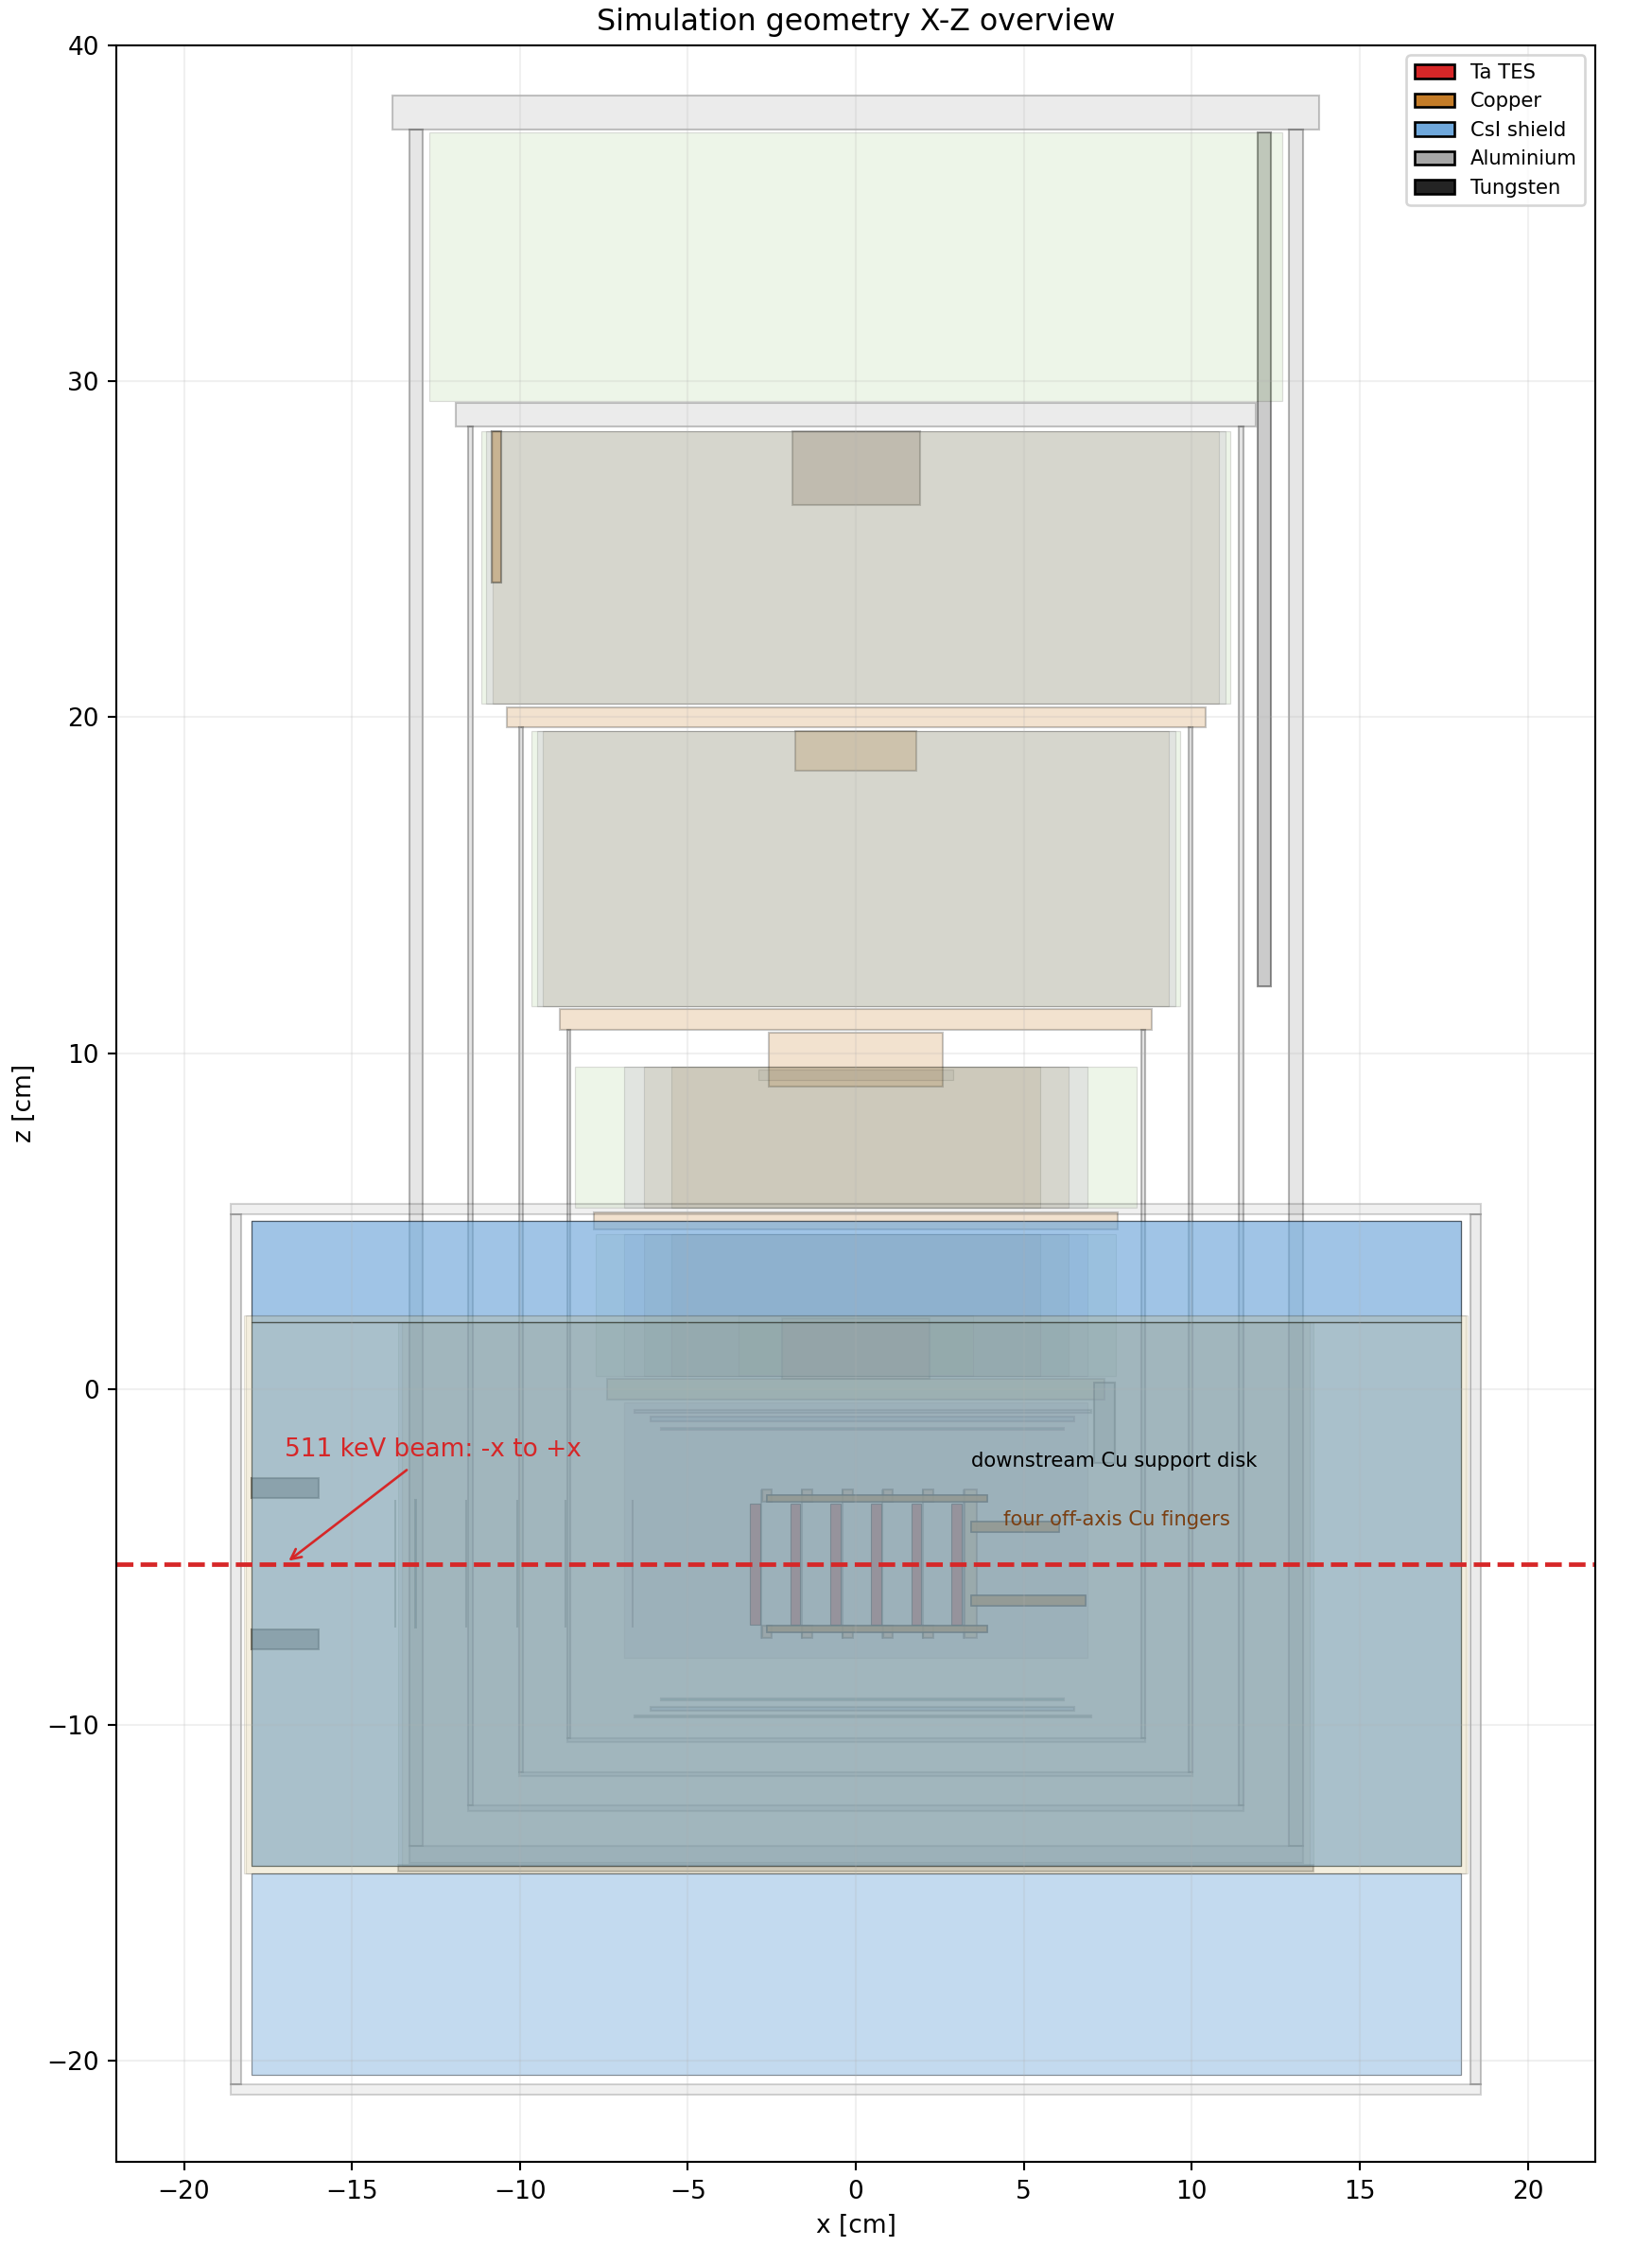
\includegraphics[width=0.62\linewidth]{paper_source_figure_table/fig_mass_model_xz_overview.png}

\vspace{0.6ex}
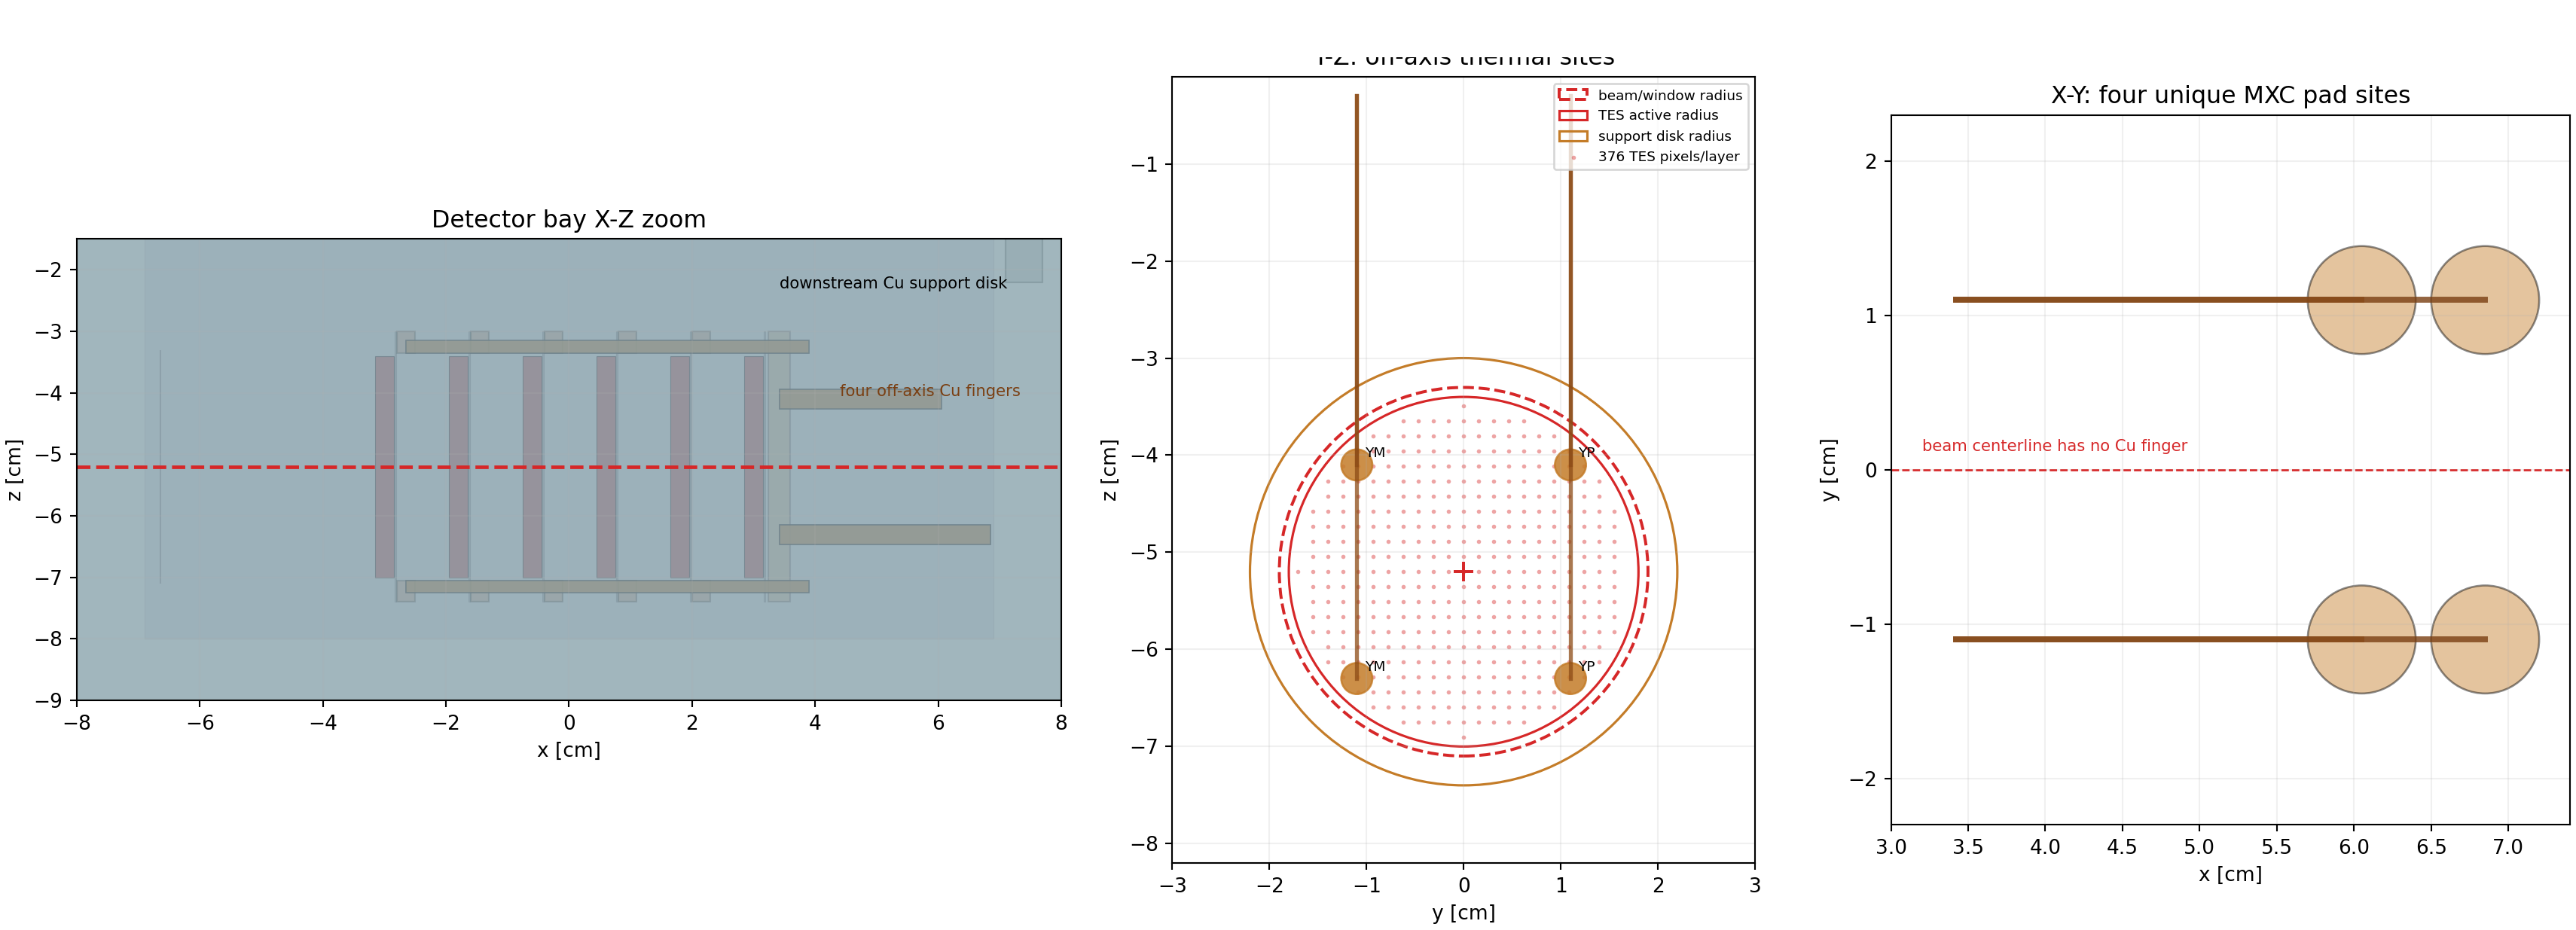
\includegraphics[width=0.88\linewidth]{paper_source_figure_table/fig_mass_model_detector_bay_detail.png}
\caption{探测器/低温系统代理质量模型的二维示意图。上：DR 塔、探测器舱、主动屏蔽和 511 keV 侧入射束线的 X--Z 视图。下：探测器舱细节，显示 TES 吸收体堆栈、开放中心束区和离轴 Cu 热连接。}
\label{fig:mass_model}
\end{figure}
\section{模拟框架}
\label{sec:framework}

通过详细质量模型的探测器耦合 Monte Carlo 输运，是预测伽马射线谱仪响应和本底的成熟方法 \cite{Sturner2003}。本节描述从源生成到飞行性能评估的整条端到端模拟链。聚焦光学和探测器系统从独立的质量模型中起步：光学分支定义的质量模型输入待观测信号点源、瞬发本底和延时本底源，然后记录通过其输运到达焦平面所在平面的所有粒子，作为探测器分支的输入聚焦源；探测器分支则在第~\ref{sec:geometry}~节的探测器/低温系统质量模型中直接输运瞬发大气粒子，以及活化产物按记录产生位置生成的延迟衰变，以及上述提及的聚焦源。聚焦源、瞬发源、延时源分步模拟，通过基于泊松统计的时间轴抽样再归一方式归一到一个时间轴里，再经由基于闪烁体的主动 veto 和基于康普顿运动学的 veto 进一步抑制本底，随后依次进入详细本底分析统计、任务飞行时间轨迹变化带来的信号本底强度变化分析，来给出整体飞行性能评估与设计优化建议。正因为聚焦信号与两路本底在任何本底分解或灵敏度陈述之前都通过了这同一套响应和 veto，后续结果才落在一致的事例选择之上。

图~\ref{fig:workflow} 把这条链路按计算层级展开：几何定义、瞬发与活化积累输运、延迟源构建、聚焦光学输运、探测器耦合信号重放、veto 机制、本底细节分析、时间/飞行轨迹变化，以及飞行性能评估与设计优化意见——下文逐层详细说明各层的输入、操作与输出。

\begin{figure}[t]
\centering
\begin{tikzpicture}[
  box/.style={rectangle, rounded corners=2pt, draw=black!55, line width=0.4pt,
              align=center, font=\scriptsize, text width=30mm, minimum height=8mm, inner sep=2pt},
  bg/.style={box, fill=blue!8},
  sig/.style={box, fill=green!12},
  shr/.style={box, fill=black!6},
  flow/.style={-{Latex[length=2mm]}, draw=black!60, line width=0.5pt}
]
\node[shr] (geo)    at (0,0)        {几何 / 质量模型};
\node[bg]  (prompt) at (-3.1,-1.35) {瞬发与活化输运};
\node[bg]  (delay)  at (-3.1,-2.7)  {延迟活度源};
\node[bg]  (decay)  at (-3.1,-4.05) {产生位置衰变输运};
\node[sig] (optics) at (3.1,-1.35)  {Laue 光学（仅信号）};
\node[sig] (couple) at (3.1,-2.7)   {光学--探测器耦合};
\node[shr] (sel)    at (0,-5.4)     {veto 机制：闪烁体 veto $+$ 康普顿运动学 veto};
\node[shr] (detail) at (0,-6.75)    {本底细节分析};
\node[shr] (fold)   at (0,-8.1)     {时间/飞行轨迹变化};
\node[shr] (out)    at (0,-9.45)    {飞行性能评估，设计优化意见};
\draw[flow] (geo) -- (prompt);
\draw[flow] (geo) -- (optics);
\draw[flow] (prompt) -- (delay);
\draw[flow] (delay) -- (decay);
\draw[flow] (optics) -- (couple);
\draw[flow] (decay) -- (sel);
\draw[flow] (couple) -- (sel);
\draw[flow] (sel) -- (detail);
\draw[flow] (detail) -- (fold);
\draw[flow] (fold) -- (out);
\end{tikzpicture}
\caption{本文采用的模拟链。蓝色节点为瞬发与延迟本底流，绿色节点为聚焦信号光学，灰色节点为共享的几何、veto 机制、本底细节分析、时间/飞行轨迹变化以及最终飞行性能评估。聚焦信号和全部本底流先在同一探测器响应与 veto 定义下评估，再用于本底分解、任务时间变化和设计优化判断。}
\label{fig:workflow}
\end{figure}

\FloatBarrier

\subsection{Laue 光学与探测器耦合信号重放}
\label{sec:optics}

本文模拟采用了基于mosaic Ge(111)晶体的laue透镜系统 \cite{Barriere2009Laue,Barriere2011LauePrototype}，通过光学设计，实现10m的焦距，\textcolor{red}{多环系统实现450keV-550keV的探测能段}，511keV下20cm**2的有效面积；有效面积按
\begin{equation}
  A_{\mathrm{eff}}(E)=A_{\mathrm{inc}}\frac{N_{\mathrm{fp}}(E)}{N_{\mathrm{inc}}(E)}
  \label{eq:laue_aeff}
\end{equation}
计算，其中 $A_{\mathrm{inc}}$ 为蒙特卡洛入射采样面积，$N_{\mathrm{inc}}(E)$ 为入射光子数，$N_{\mathrm{fp}}(E)$ 为满足聚焦/焦面截取条件的光子数。
采用mosaic系统是为了在满足预期设计的聚焦性能前提下便于蒙特卡洛计算，实际工程适配时也有其他候选方案。

在本模拟中，laue光学分支除了给出了聚焦性能模拟，\textcolor{red}{也实现了本身作为质量的粒子输运模拟}。

为此,晶体对光子的衍射概率不再作为一个效率参数叠加给光子,而是在 Geant4 应用层定义为一个离散过程 \cite{Agostinelli2003,Allison2016}。该过程按当前光子相对晶面的角偏差取衍射概率 $R(|\Delta\theta|)$,并把它转换为一个有限的等效衍射平均自由程 $\lambda_{\mathrm{diff}}$,使光子穿过晶体路径 $\ell$ 时累计的衍射概率复现该值:$1-\exp(-\ell/\lambda_{\mathrm{diff}})=R(|\Delta\theta|)$,即 $\lambda_{\mathrm{diff}}=-\,\ell/\ln[1-R(|\Delta\theta|)]$;为避免与标准光电吸收重复计数,$R$ 先按未吸收份额归一($R/(1-A)$)再转成自由程。该自由程交回 Geant4 后,衍射过程与标准电磁过程(光电吸收、康普顿散射)在同一竞争框架下各自抽样相互作用长度,由最短者决定谁先发生,而不是在晶体边界强制拦截光子。未被抽中发生衍射的光子仍按标准电磁物理继续输运,可能被吸收、散射或直接透射。

衍射概率优先由外部 XOP/CRYSTAL rocking-curve map 按角偏差插值给出:该曲线由 XOP 工具包的 CRYSTAL/diff\_pat 模块(经 xoppylib 调用,以 DABAX 晶体学数据为输入)在预处理阶段一次性离线计算 \cite{SanchezDelRio2011XOP},给出 Ge(111) 反射率/透射率/吸收随角偏差的曲线;输运过程中对晶体内每一步实时计算角偏差,在该曲线上插值取当前衍射概率,即“库离线建表、概率随输运按角取用”。mosaic 取向通过对理想 Bragg 晶面法线施加高斯角扰动实现,扰动宽度由 30 角秒 mosaic FWHM 给出;衍射发生后,出射方向按扰动后的晶面法线镜面反射,光子能量不变。这种“过程类只负责输运接口、独立模型类负责概率与方向判定”的拆分方式,借鉴了 Geant4 中已有的晶体 Bragg 反射扩展工作的思路 \cite{Guan2023BraggReflection,Reiazi2025G4BraggReflection}，扩展到我们所需能段。

这里的参考信号是一个单色 511 keV点源，其通量尺度并非取自某个特定天体，而是由叠加在银心弥散辐射之上的致密 511 keV点源的 INTEGRAL/SPI 上限设定（大气层上 $\fzero=10^{-4}\phcms$，见第~\ref{sec:geometry} 节）\cite{Siegert2016AA,DeCesare2011}。信号以 megalib 远场源方式构建 \cite{Zoglauer2006}，详细构建方式见第~\ref{subsec:pointsource} 节。除信号外，我们还以远场源方式构建宇宙线瞬发本底与活化本底。上述三种源的输运分别模拟；每次模拟均截取穿过焦平面所在平面的粒子通量、种类与能量作为输出，按等效观测时间归一化后，作为一个平行束源输入探测器的质量模型。

\subsection{源构建}
\label{sec:background}

在第~\ref{sec:optics} 节定义了聚焦光学之后，光学输入及后续探测器输入还需要三层源：
入射到载荷上的瞬发大气粒子场，该粒子场在仪器中积累起来的延迟放射性群体，以及用于
参考的信号点源。三者分开构建，而不是直接调用 MEGAlib 的 buildup 功能同时跑输运，
这样是为了节约计算成本。

\subsubsection{瞬发大气源}
\label{subsec:prompt_source}

瞬发大气粒子场由 EXPACS/PARMA 给出。PARMA3.0 是由 PHITS 大气级联计算参数化得到、
并针对陆地宇宙线测量验证过的解析模型，EXPACS 是其公开表格与软件接口
\cite{Sato2015EXPACS,Sato2016PARMA4}。底层的粒子输运物理由 PHITS 提供：一次宇宙线
与大气核作用，次级强子、轻子、光子和中子在大气柱中继续输运，最终通量按海拔、
地磁截止刚度、太阳调制、能量和方向参数化。本文中 EXPACS/PARMA 给出随粒子种类、
动能、天顶角、地理位置、海拔、截止刚度和太阳活动变化的入射微分通量，且只用于构造
外部辐射场；探测器响应、反符合、拓扑选择和任务时间计数都在下游施加。参考源定义
采用纬度 $34^\circ$、经度 $100^\circ$、海拔 $38\,\mathrm{km}$、垂直截止刚度
$R_c=11.6\,\mathrm{GV}$，以及 2025-08-31 对应的太阳条件 $W=118.3$。

瞬发源包含光子、中子、电子、正电子、质子、$\alpha$ 粒子以及正负 $\mu$ 子。对每个
粒子族，EXPACS/PARMA 微分谱被转换为 MEGAlib 远场面积源，覆盖完整天顶角范围
$\theta=0^\circ$--$180^\circ$ 和完整方位角范围 $\phi=0^\circ$--$360^\circ$。天顶角
依赖用 20 个等 $\mu$ 微分分箱表示，其中 $\mu=\cos\theta$，每箱立体角
$\Delta\Omega=0.6283185307\,\mathrm{sr}$：前 10 箱为下行粒子，后 10 箱为上行或反照
成分。瞬发输运和活化产生输运都保留这两个半球，因此源构建阶段没有丢弃上行反照
粒子。图~\ref{fig:expacs_fullsphere_flux} 给出由源定义实际采用的全空间通量场。

\begin{figure}[t]
\centering
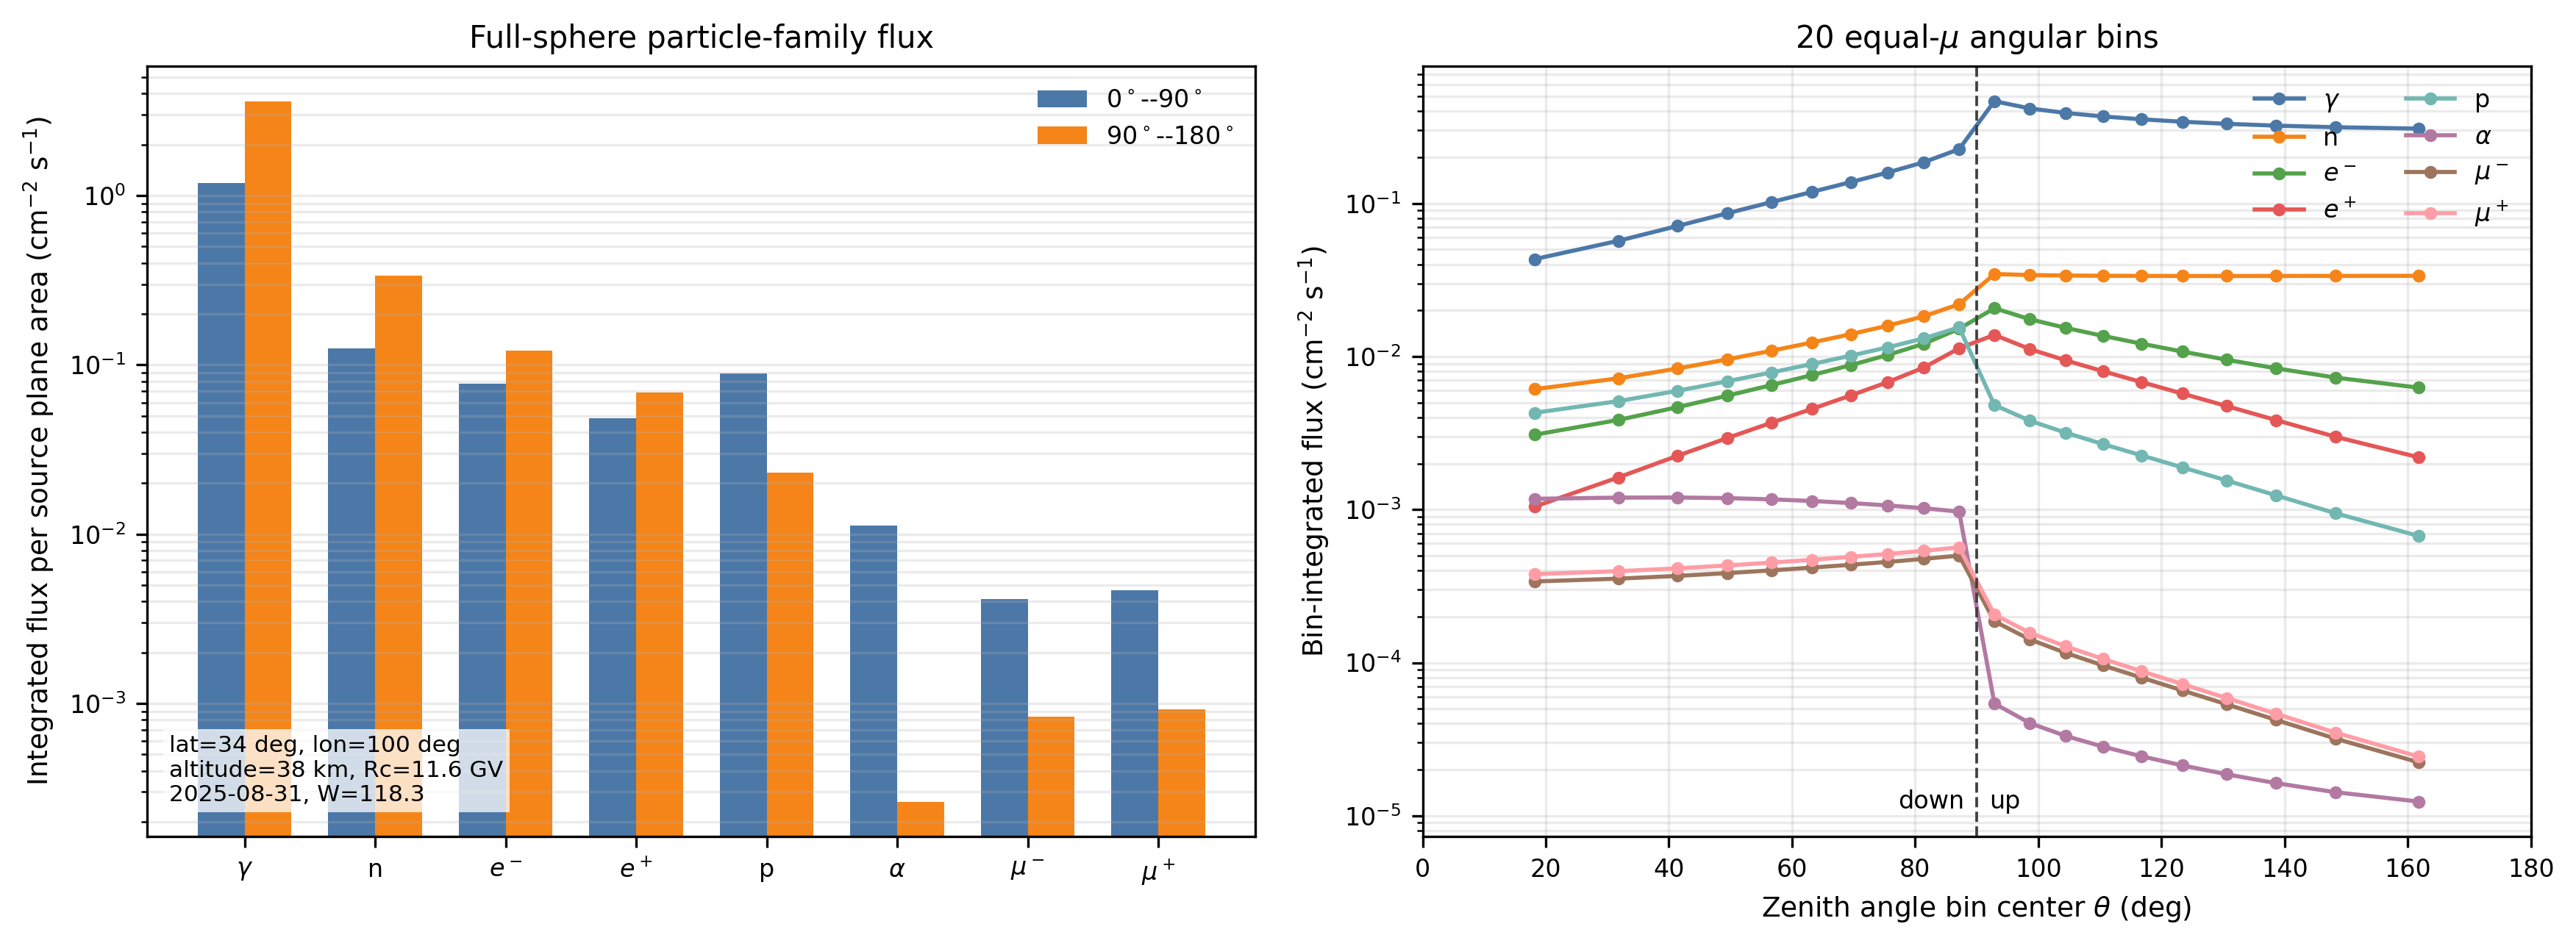
\includegraphics[width=\linewidth]{paper_source_figure_table/fig_expacs_fullsphere_flux.png}
\caption{用于生成瞬发和活化产生输运输入的 EXPACS/PARMA 全空间大气通量场。左：八类输运粒子族的能量和立体角积分通量，并按下行、上行半球分开。右：MEGAlib 远场源使用的 20 个等 $\mu$ 微分天顶角分箱的积分通量。该图直接由源定义输入表生成，环境参数为纬度 $34^\circ$、经度 $100^\circ$、海拔 $38\,\mathrm{km}$、$R_c=11.6\,\mathrm{GV}$、$W=118.3$。}
\label{fig:expacs_fullsphere_flux}
\end{figure}

积分源面通量约为 $4.80$、$0.462$、$0.199$、$0.117$、$0.112$、$0.0115$、$0.0050$
和 $0.0056\,\mathrm{cm^{-2}\,s^{-1}}$，分别对应 $\gamma$、$n$、$e^-$、$e^+$、$p$、
$\alpha$、$\mu^-$ 和 $\mu^+$；非光子成分合计约 $0.91\,\mathrm{cm^{-2}\,s^{-1}}$，
占全空间源面积分通量的 16\%。若严格按通量比例分配蒙特卡洛计数，这些少数粒子族的
探测器命中和活化统计将很差，因此非光子粒子族采用复制样本生成，再在率归一化中
去权重。随后所有粒子经 Geant4/MEGAlib 在探测器/低温系统质量模型中输运
\cite{Agostinelli2003,Allison2016,Zoglauer2006}；瞬发流和活化产生流各生成
25{,}210{,}216 个入射一次粒子。每个粒子种类用自身输运曝光归一：
\begin{equation}
  r_{\mathrm{event},j}=\left(\sum_i \mathcal{T}_{ij}\right)^{-1},
\end{equation}
其中 $\mathcal{T}_{ij}$ 为粒子种类 $j$ 在输运子样本 $i$ 中的曝光。由于光子流和
非光子流的采样与曝光结构不同，这种按种类归一是必要的；归一化检查要求每个种类满足
$r_{\mathrm{event},j}\sum_i\mathcal{T}_{ij}=1$，因此过采样只改变蒙特卡洛方差，
不改变物理期望率。

\subsubsection{延迟活化源}
\label{subsec:delayed_source}

对于延迟模拟，则另外跑一个活化产生流，方法是在瞬发本底输运中打开 BUILDUP。活化
产生流不作为即时探测器本底计数，而是记录每个放射性产物的核素、材料体积和产生位置。
这些记录通过产生--衰变积累方程转换为固定到飞行过程中某一参考时刻的放射性群体，
基态半衰期已对照 NUBASE2020 校验 \cite{Kondev2021NUBASE}。对核素 $k$，
\begin{equation}
  A_k(t_{\mathrm{flight}}) = P_k\left[1-\exp\left(-\lambda_k t_{\mathrm{flight}}\right)\right],
  \qquad \lambda_k = \frac{\ln 2}{t_{1/2,k}},
\end{equation}
其中 $P_k$ 是由活化产生输运推得的产生率，参考状态取 $t_{\mathrm{flight}}=15\,\mathrm{d}$。
参考延迟源构建使用的固定延迟总活度为 $85.45\,\mathrm{Bq}$。

位置信息并非只来自聚合后的同位素清单。标准清单记录产生体积和核素计数；产生位置
构建另在 MEGAlib 的 stepping-action 层加入自定义记录钩子：在活化积累模式中
每存入一个延迟核素，钩子就在同一时刻写出一条产生位置记录，包含逻辑体名称、
pre-step 位置 $(x,y,z)$、核素编号 $1000Z+A$、激发能、时间、过程和 track ancestry
信息。固定第 15 天群体随后按体积、核素和激发态与这些记录匹配，使延迟源能够使用
模拟产生坐标，而不是只有体积积分活度。附录~\ref{app:delayed} 中的
图~\ref{fig:delayed_position_distribution} 给出匹配后的位置分布：活度加权分布以
CsI 屏蔽活化和 $^{128}$I 为主，Cu、Al、W、Mg 和 Cs 等核素贡献较小。该图是源构建
诊断图而非探测器计数图；探测器响应只有在延迟衰变经过共同几何和共同事例选择输运
之后才施加。

产生位置是否值得保留，可以直接用同一张产生表检验。延迟衰变在局部材料中发射，
下游衰减、主动屏蔽 veto 概率和事例拓扑都取决于核素产生在哪里；而不同入射粒子族
的能量损失、停止和俘获历史不同，其活化产物也不必落在相同的材料里。为量化这一点，
把加权产生行按入射粒子族和材料类别分组，用 total-variation 距离比较两个粒子族
$a$、$b$ 的活度归一化材料分布：
\begin{equation}
  D_{\mathrm{TV}}(a,b) =
  \frac{1}{2}\sum_c \left| f_{a,c} - f_{b,c} \right| ,
\end{equation}
其中 $f_{a,c}$ 为入射族 $a$ 在材料类别 $c$ 中产生的延迟活度占比。在固定第 15 天
表中，中子诱发产物约 $82.5\,\mathrm{Bq}$，$\mu^-$ 诱发产物 $2.75\,\mathrm{Bq}$，
质子诱发产物 $0.15\,\mathrm{Bq}$，$\alpha$ 诱发产物 $0.022\,\mathrm{Bq}$，另有更小
的 $\mu^+$ 和 $e^+$ 项。中子诱发活度仍以 CsI 屏蔽为主，而 $\mu^-$ 成分则明显不同：
Cu/支撑材料、Al 壳层和含 W 被动材料分别占 $\mu^-$ 诱发活度的 32\%、29\% 和 21\%
（附录~\ref{app:delayed} 图~\ref{fig:position_sampling_necessity}）。体积积分源或
轴对称径向源可以保住总活度，却会抹掉这些入射族--材料--核素--坐标之间的相关性；
产生位置构建把它们保留在进入探测器输运之前的源里。

延迟衰变源因此从采样的产生位置发射，而不是从轴对称分布发射。设加权产生表第 $j$
行的活度权重为 $w_j$，总活度 $A=\sum_j w_j$。构建时以 $p_j=w_j/A$ 为概率有放回
抽取 $M$ 个产生位置，并给每个采样点源相同通量 $A/M$，则第 $j$ 行获得的期望活度为
\begin{equation}
  \mathbb{E}\!\left[N_j\frac{A}{M}\right] = M p_j \frac{A}{M} = w_j ,
\end{equation}
即该估计保持总活度，并对加权空间分布无偏。这里 $M$ 是等活度采样点源的数目，是
采样规模而不是物理产生行数。参考延迟源在源定义层面保持固定总活度，并在与瞬发流
相同的探测器/低温系统几何中重放；名义计算输运 $10^{6}$ 个延迟衰变，相应的 Cosima
live time 只是生成衰变序列的输运记录，不作为物理气球曝光时间使用。

表~\ref{tab:background_source_model} 汇总了当前探测器耦合计算使用的源层级。它放在
源模型部分，是因为这里定义的是入射粒子场和延迟放射性群体；探测器 veto 和拓扑选择
都在后续选择部分才施加。

\begin{table}[t]
\centering
\caption{当前探测器耦合链路中的本底源分层。表中只定义源构建；反符合、拓扑筛选和线窗在第~\ref{sec:selection} 节才施加。}
\label{tab:background_source_model}
\begin{tabular}{p{0.22\linewidth}p{0.34\linewidth}p{0.34\linewidth}}
\hline
层级 & 物理作用 & 当前实现 \\
\hline
瞬发大气输运 & 大气次级粒子造成的直接探测器命中 & EXPACS/PARMA 全空间源定义，环境为纬度 $34^\circ$、经度 $100^\circ$、海拔 $38\,\mathrm{km}$、$R_c=11.6\,\mathrm{GV}$、$W=118.3$；$\gamma$、$n$、$e^\pm$、$p$、$\alpha$ 和 $\mu^\pm$ 覆盖 20 个等 $\mu$ 微分天顶角分箱，并同时包含下行和上行半球；生成 25,210,216 个入射一次粒子。 \\
活化产生 & 放射性核素产生及其产生位置历史 & 在瞬发本底输运中打开 BUILDUP 得到活化产生流，同样保留两个半球和八类粒子族；生成 25,210,216 个入射一次粒子。 \\
固定延迟放射性群体 & 连续曝光后采用的第 15 天状态放射性活度 & 产生--衰变积累，并用 NUBASE 校验的基态半衰期修正；总固定活度 $85.45\,\mathrm{Bq}$。 \\
产生位置衰变输运 & 延迟衰变粒子从采样产生位置发射 & 从加权产生表得到等活度采样点源；参考输运对每个源采样输运 $10^6$ 个延迟衰变。 \\
\hline
\end{tabular}
\end{table}

该产生位置表示并非对每条产生行都建立一个采样点源，而是一种统计采样近似，其充分性
在第~\ref{subsec:convergence} 节的选后率层面另行评估。源清单检查用于核对活度守恒
和源序列化；选后率行为则在探测器输运和事例选择之后单独检验。

\subsubsection{参考点源构建}
\label{subsec:pointsource}

聚焦信号流由一个单色 511 keV参考点源定义。其通量尺度不取自某个特定天体，而是由
叠加在银心弥散辐射之上的致密 511 keV点源的 INTEGRAL/SPI 上限设定，即大气层上
$\fzero=10^{-4}\phcms$（见第~\ref{sec:geometry} 节）\cite{Siegert2016AA,DeCesare2011}。

由于此类源位于天文距离处，它被建模为理想的轴上点源：在光学 run 中它是一束单色
511 keV远场光束，光子平行于光轴入射，并在式~(\ref{eq:laue_aeff}) 的入射孔径
$A_{\mathrm{inc}}$ 上均匀采样。源本身不赋予有限角尺寸；到达焦面的角结构完全由透镜
产生——30 角秒 mosaic 展宽、XOP/CRYSTAL 摇摆曲线，以及 $f=10\,\mathrm{m}$ 聚焦
几何——因此重放束收敛在离轴约 $0.4^\circ$ 内，形成聚焦斑而非单条光线。三个独立种子
各 $5\times10^{4}$ 个一次粒子，共 $1.5\times10^{5}$ 个输运光子，其中 37{,}256 个发生
衍射并穿过焦面；这些光子中 37{,}194 个（99.8\%）落在 $r=1.898\,\mathrm{cm}$ 的 Be
入射窗内，聚焦斑半径 $r_{90}=1.03\,\mathrm{cm}$、$r_{99}=1.25\,\mathrm{cm}$。窗内穿越
构成事件表，按记录的位置与方向经 Be 孔径重放进探测器/低温系统模型。

归一化把该重放接回参考通量。探测器入口处聚焦流的率为 $\fzero\,\aeff(511\keV)\,T$，
其中 $\aeff(511\keV)=20.1\,\mathrm{cm^2}$ 为轴上有效面积，$T=0.739$ 为第 15 天轨迹锚
点处 511 keV的参考大气透过率；在参考通量下数值为 $1.48\times10^{-3}\cps$。等价地，
生成 run 对应观测时间 $N_{\mathrm{fp}}/[\fzero\,\aeff\,T]$，每个重放事件以该曝光的倒数
作为率权重；在第~\ref{sec:selection} 节的中间 cut-flow 记账中，同一样本在施加该尺度前
以单位重放出现。经过共同的探测器响应与事例选择后，存活信号率为
$1.19\times10^{-3}\cps$，对应选后有效面积 $S_{\wii}/\fzero=11.9\,\mathrm{cm^2}$。由于
光学 run 只含源光子，重放流是信号纯净的；所有本底均通过第~\ref{sec:background} 节的
各源流引入。

上文引用的有效面积为轴上值，代表最佳指向情形。点源偏离光轴、或飞行中的残余姿态抖动，
会通过 Laue 透镜有限的角接受（视场）降低并移动聚焦响应
\cite{Barriere2009Laue,Weidenspointner2006MAX}；这一离轴依赖作为对信号有效面积的指向
系统学处理，而不改变轴上参考构建。

\subsection{探测器事例选择与 veto 定义}
\label{sec:selection}


\added{为把这一选择链路和有限 Monte Carlo 统计显式对应起来，表~\ref{tab:phase2_cutflow} 给出当前 事例级 证据包从 事例选择 事例目录轻量解析得到的 $\wii$ cut-flow。该表不来自新的 Geant4/MEGAlib 输运，而是对当前事例目录按相同 TES 能窗、CsI veto 和康普顿运动学/视场一致性检验重放；不确定度为按事例权重做的 Monte Carlo 二次和。当前 事例选择 记录先固定能窗再记录 raw、主动屏蔽和拓扑阶段，因此表中的 raw 阶段应理解为线窗内预 veto 样本，而不是全能段入射样本。}

% [RECOVERY GAP: original lines 319-319 not found in logs]
则通过主动屏蔽。基准 CsI 配置中的屏蔽能量由 CsI 主动屏蔽体积
在后处理中读取。几何描述中存在探测器触发和 veto 标记，但定量率
定义采用这里的统一后处理定义，因此瞬发、延迟和聚焦信号流使用相同的
coincidence 窗和阈值。

第二层是对主动屏蔽通过后的 TES 命中施加拓扑/视场一致性检验。基准事例类别保持显式区分：单点事例、有效重建的多点事例和未重建的多点事例。
单像素 TES 事例作为量热线候选保留。双命中事例测试两个可能的第一散射顺序。对一个
假定顺序，若第一沉积能量为 $E_1$、剩余散射光子能量为
$E_{\mathrm{sc}}$，则运动学散射角由
\begin{equation}
  \cos\theta_C =
  1 - m_ec^2\left(\frac{1}{E_{\mathrm{sc}}}
  - \frac{1}{E_1+E_{\mathrm{sc}}}\right)
\end{equation}
给出。若任一顺序给出物理有效的第一散射锥并与侧入射 Be 窗圆盘相交，
则该事例保留。对更高多重度事例，当前实现枚举最多六个 TES 命中的候选
顺序，并用常用的康普顿序列残差
\begin{equation}
  Q = \sum_{i=1}^{n-2}
  \left(\cos\theta_{C,i} -
  \hat{\mathbf u}_{i-1,i}\cdot\hat{\mathbf u}_{i,i+1}\right)^2
\end{equation}
选择最佳顺序，然后对第一散射锥施加同一窗口相交检验。若没有有效顺序，
该事例被归为未重建类。此类事例在基准选后率定义中保留，但不称为通过视场的事例。因此本文线窗结果没有从剔除歧义重建失败事例中获得灵敏度增益。
该策略并不是净灵敏度的保守下界。诊断性替代选择表明，如果采用
single-site-only 口径并把所有多命中候选作为 veto 丢弃，在当前 $\wii$
样本中会保留 $59.4\%$ 的聚焦信号和 $68.2\%$ 的选后本底，并把简单
$S/\sqrt{B}$ 降低到基准值的 $0.720$。因此，基准选择把歧义多命中事例视为一个需要后续重建验证的
模型边界，而不是把激进事例拒绝作为灵敏度增益来源。

\added{为把这一选择链路和有限 Monte Carlo 统计显式对应起来，表~\ref{tab:phase2_cutflow} 给出当前 事例级 证据包从 事例选择 事例目录轻量解析得到的 $\wii$ cut-flow。该表不来自新的 Geant4/MEGAlib 输运，而是对当前事例目录按相同 TES 能窗、CsI veto 和康普顿运动学/视场一致性检验重放；不确定度为按事例权重做的 Monte Carlo 二次和。当前 事例选择 记录先固定能窗再记录 raw、主动屏蔽和拓扑阶段，因此表中的 raw 阶段应理解为线窗内预 veto 样本，而不是全能段入射样本。}

\begin{table}[t]
\centering
\caption{\added{事例级 证据包给出的 $\wii$ 线窗 cut-flow。}}
\label{tab:phase2_cutflow}
\footnotesize
\resizebox{\linewidth}{!}{%
{
\begin{tabular}{llccc}
\toprule
流 & 阶段 & 事例数 & 率 / $\cps$ & 统计不确定度 / $\cps$ \\
\midrule
瞬发本底 & 线窗预 veto & 161 & $1.1877\times10^{-1}$ & $1.15\times10^{-2}$ \\
瞬发本底 & CsI veto 后 & 60 & $4.0712\times10^{-2}$ & $5.26\times10^{-3}$ \\
瞬发本底 & 拓扑/视场选后 & 54 & $3.6641\times10^{-2}$ & $4.99\times10^{-3}$ \\
延迟活化 & 线窗预 veto & 54 & $4.6354\times10^{-3}$ & $6.31\times10^{-4}$ \\
延迟活化 & CsI veto 后 & 33 & $2.8327\times10^{-3}$ & $4.93\times10^{-4}$ \\
延迟活化 & 拓扑/视场选后 & 30 & $2.5752\times10^{-3}$ & $4.70\times10^{-4}$ \\
聚焦信号 & 线窗预 veto & 30323 & $8.1527\times10^{-1}$ & $4.68\times10^{-3}$ \\
聚焦信号 & CsI veto 后 & 30323 & $8.1527\times10^{-1}$ & $4.68\times10^{-3}$ \\
聚焦信号 & 拓扑/视场选后 & 29715 & $7.9892\times10^{-1}$ & $4.63\times10^{-3}$ \\
\bottomrule
\end{tabular}
}}
\vspace{0.5ex}
\begin{minipage}{0.94\linewidth}
\footnotesize
聚焦信号行是 事例选择 事例目录中的单位重放率，用于说明 veto 保留行为；表~\ref{tab:primary_sensitivity} 中的点源信号率另按 Laue 有效面积、参考通量和大气透过率缩放。
\end{minipage}
\end{table}
% [RECOVERY GAP: original lines 381-635 not found in logs]

\rewritten{在该率级研究能够支撑飞行性能声明之前，仍有四类验证需要完成：保留多命中子样本的 Revan/Mimrec 或等价重建交叉检查，并给出残差分布和阈值稳定性；包含明确透镜晶片和支撑硬件的全统计量光学硬件自本底输运；最终低温/DR 几何和探测器响应更新，其中包括 TES 饱和与堆积约束；以及可对本底扰动参数做剖面化处理的空间--谱联合似然。当前红字补充的 事例级 表格应理解为这些验证之前的论文支撑证据和审计入口，而不是完整系统误差包络。}

\subsection{结论}
\label{sec:conclusions}

本文给出了气球载指向式 511 keV TES Laue 透镜望远镜的探测器耦合本底和灵敏度研究。参考计算把 Ge(111) Laue 光学响应与 TES 焦平面质量模型、瞬发大气输运、延迟活化、主动屏蔽 veto、拓扑/视场选择、任务时间率折叠和计数显著度评估结合起来。在主要 $510.79$--$511.21\keV$ 未分辨线窗中，第 15 天选后率为 $B\simeq3.92\times10^{-2}\cps$，对 $10^{-4}\phcms$ 参考点源有 $S\simeq1.19\times10^{-3}\cps$；任务时间折叠后得到 $Z_{20\mathrm{d}}\simeq7.80$ 和 $\fthree(20\mathrm{d})\simeq3.85\times10^{-5}\phcms$。该结果为继续评估聚焦式 TES 谱学作为 511 keV 紧凑源和未分辨中央增强搜索的互补技术提供了探测器耦合选后率依据，同时指出瞬发大气本底抑制、延迟活化系统误差验证和重建验证是下一阶段的主要验证任务。


\clearpage
\section*{恢复缺口说明}
原始日志片段在第 381--635 行和附录/参考文献附近存在缺口。本文件只生成可阅读 PDF，缺失正文请继续从恢复片段或人工补稿。

\begin{thebibliography}{99}

\bibitem{Prantzos2011}
N. Prantzos, C. Boehm, A.M. Bykov, R. Diehl, K. Ferriere, N. Guessoum, P. Jean, J. Knoedlseder, A. Marcowith, I.V. Moskalenko, A. Strong, G. Weidenspointner, The 511 keV emission from positron annihilation in the Galaxy, Rev. Mod. Phys. 83 (2011) 1001--1056, doi:10.1103/RevModPhys.83.1001.

\bibitem{Jean2006}
P. Jean, J. Knoedlseder, V. Lonjou, M. Allain, J.-P. Roques, G.K. Skinner, B.J. Teegarden, G. Vedrenne, P. von Ballmoos, B. Cordier, P. Caraveo, R. Diehl, P. Durouchoux, P. Leleux, R. Schanne, G. Weidenspointner, Spectral analysis of the Galactic $e^+e^-$ annihilation emission, Astron. Astrophys. 445 (2006) 579--589, doi:10.1051/0004-6361:20053765.

\bibitem{Siegert2016AA}
T. Siegert, R. Diehl, G. Khachatryan, M.G.H. Krause, F. Guglielmetti, J. Greiner, A.W. Strong, X. Zhang, Gamma-ray spectroscopy of positron annihilation in the Milky Way, Astron. Astrophys. 586 (2016) A84, doi:10.1051/0004-6361/201527510.

\bibitem{Siegert2019Kinematics}
T. Siegert, R. Diehl, G. Khachatryan, M.G.H. Krause, F. Guglielmetti, J. Greiner, A.W. Strong, X. Zhang, Constraints on positron annihilation kinematics in the inner Galaxy, Astron. Astrophys. 627 (2019) A126, doi:10.1051/0004-6361/201833856.

\bibitem{Yoneda2025}
H. Yoneda, T. Siegert, S. Mittal, Imaging the positron annihilation line with 20 years of INTEGRAL/SPI observations, arXiv:2509.01066, 2025.

\bibitem{Kierans2020}
C.A. Kierans, S.E. Boggs, A. Zoglauer, A.W. Lowell, C. Sleator, J. Beechert, T.J. Brandt, P. Jean, H. Lazar, J. Roberts, T. Siegert, J.A. Tomsick, P. von Ballmoos, Detection of the 511 keV Galactic positron annihilation line with COSI, Astrophys. J. 895 (2020) 44, doi:10.3847/1538-4357/ab89a9.

\bibitem{Siegert2020COSI}
T. Siegert, S.E. Boggs, J.A. Tomsick, A.C. Zoglauer, C.A. Kierans, C.C. Sleator, J. Beechert, T.J. Brandt, P. Jean, H. Lazar, A.W. Lowell, J.M. Roberts, P. von Ballmoos, Imaging the 511 keV positron annihilation sky with COSI, Astrophys. J. 897 (2020) 45, doi:10.3847/1538-4357/ab9607.

\bibitem{Siegert2016V404}
T. Siegert, R. Diehl, J. Greiner, M.G.H. Krause, A.M. Beloborodov, M. Cadolle Bel, F. Guglielmetti, J. Rodriguez, A.W. Strong, X. Zhang, Positron annihilation signatures associated with the outburst of the microquasar V404 Cygni, Nature 531 (2016) 341--343, doi:10.1038/nature16978.

\bibitem{DeCesare2011}
G. De Cesare, Searching for the 511 keV annihilation line from galactic compact objects with the IBIS gamma ray telescope, Astron. Astrophys. 531 (2011) A56, doi:10.1051/0004-6361/201116516.

\bibitem{Roques2015}
J.-P. Roques, E. Jourdain, A. Bazzano, A. Fiocchi, A. Bazzano, M. Del Santo, First INTEGRAL observations of V404 Cygni during the 2015 outburst: spectral behavior in the 20--650 keV energy range, Astrophys. J. Lett. 813 (2015) L22, doi:10.1088/2041-8205/813/1/L22.

\bibitem{Shirazi2023}
F. Shirazi, E. Gau, M.A. Hossen, D. Becker, D. Schmidt, D. Swetz, D. Bennett, D. Braun, F. Kislat, J. Gard, J. Mates, J. Weber, N.R. Cavero, S. Chun, L. Lisalda, A. West, B. Dev, F. Ferrer, R. Bose, J. Ullom, H. Krawczynski, The 511-CAM Mission: A pointed 511 keV gamma-ray telescope with a focal plane detector made of stacked transition edge sensor microcalorimeter arrays, J. Astron. Telesc. Instrum. Syst. 9 (2023) 024006, doi:10.1117/1.JATIS.9.2.024006.

\bibitem{Barriere2009Laue}
N.M. Barriere, L. Natalucci, N. Abrosimov, P. von Ballmoos, P. Bastie, P. Courtois, M. Jentschel, J. Knodlseder, J. Rousselle, P. Ubertini, Soft gamma-ray optics: new Laue lens design and performance estimates, arXiv:0910.0488, 2009.

\bibitem{Barriere2011LauePrototype}
N.M. Barriere, J.A. Tomsick, S.E. Boggs, A. Lowell, P. von Ballmoos, Developing a second generation Laue lens prototype: high reflectivity crystals and accurate assembly, arXiv:1111.6700, 2011.

\bibitem{Weidenspointner2006MAX}
G. Weidenspointner, C.B. Wunderer, N. Barriere, A. Zoglauer, P. von Ballmoos, Monte Carlo study of detector concepts for the MAX Laue Lens gamma-ray telescope, arXiv:astro-ph/0603152, 2006.

\bibitem{SanchezDelRio2011XOP}
M. Sanchez del Rio, R.J. Dejus, XOP v2.4: recent developments of the x-ray optics software toolkit, Proc. SPIE 8141 (2011) 814115, doi:10.1117/12.893911.

\bibitem{Gottardi2021TESReview}
L. Gottardi, K. Nagayoshi, A review of X-ray microcalorimeters based on superconducting transition edge sensors for astrophysics and particle physics, Applied Sciences 11 (2021) 3793, doi:10.3390/app11093793.

\bibitem{Zhang2022TESGamma}
S. Zhang, J.-K. Xia, T. Sun, et al., Transition edge sensor based detector: from X-ray to gamma-ray, arXiv:2204.00010, 2022.

\bibitem{Gehrels1985}
N. Gehrels, Instrumental background in balloon-borne gamma-ray spectrometers and techniques for its reduction, Nucl. Instrum. Methods Phys. Res. A 239 (1985) 324--349, doi:10.1016/0168-9002(85)90732-6.

\bibitem{Sato2015EXPACS}
T. Sato, Analytical model for estimating terrestrial cosmic ray fluxes nearly anytime and anywhere in the world: extension of PARMA/EXPACS, PLoS ONE 10 (2015) e0144679, doi:10.1371/journal.pone.0144679.

\bibitem{Sato2016PARMA4}
T. Sato, Analytical model for estimating the zenith angle dependence of terrestrial cosmic ray fluxes, PLoS ONE 11 (2016) e0160390, doi:10.1371/journal.pone.0160390.

\bibitem{Kondev2021NUBASE}
F.G. Kondev, M. Wang, W.J. Huang, S. Naimi, G. Audi, The NUBASE2020 evaluation of nuclear physics properties, Chinese Phys. C 45 (2021) 030001, doi:10.1088/1674-1137/abddae.

\bibitem{Sturner2003}
S.J. Sturner, C.R. Shrader, G. Weidenspointner, B.J. Teegarden, D. Attie, B. Cordier, R. Diehl, C. Ferguson, P. Jean, A. von Kienlin, P. Paul, F. Sanchez, S. Schanne, P. Sizun, G. Skinner, C.B. Wunderer, Monte Carlo simulations and generation of the SPI response, Astron. Astrophys. 411 (2003) L81--L84, doi:10.1051/0004-6361:20031171.

\bibitem{Agostinelli2003}
S. Agostinelli, J. Allison, K. Amako, et al., Geant4---a simulation toolkit, Nucl. Instrum. Methods Phys. Res. A 506 (2003) 250--303, doi:10.1016/S0168-9002(03)01368-8.

\bibitem{Allison2016}
J. Allison, K. Amako, J. Apostolakis, et al., Recent developments in Geant4, Nucl. Instrum. Methods Phys. Res. A 835 (2016) 186--225, doi:10.1016/j.nima.2016.06.125.

\bibitem{Zoglauer2006}
A. Zoglauer, R. Andritschke, F. Schopper, MEGAlib: The Medium Energy Gamma-ray Astronomy Library, New Astron. Rev. 50 (2006) 629--632, doi:10.1016/j.newar.2006.06.049.

\bibitem{Caputo2017}
R. Caputo, F. Kislat, J. Racusin, on behalf of the AMEGO Team, AMEGO: Simulations of the instrument performance, Proc. 35th International Cosmic Ray Conference, PoS(ICRC2017) 783 (2018), doi:10.22323/1.301.0783.

\bibitem{Karwin2023}
C.M. Karwin, T. Siegert, J. Beechert, J.A. Tomsick, T.A. Porter, M. Negro, C. Kierans, M. Ajello, I. Martinez Castellanos, A. Shih, A. Zoglauer, S.E. Boggs, Probing the Galactic diffuse continuum emission with COSI, arXiv:2310.12206, 2023.

\bibitem{Gallego2025Balloon}
S. Gallego, U. Oberlack, J. Lommler, C.M. Karwin, A. Zoglauer, P. Jean, P. von Ballmoos, C. Kierans, C.C. Sleator, J.A. Tomsick, S.E. Boggs, Bottom-up background simulations of the 2016 COSI balloon flight, arXiv:2503.02493, 2025.

\bibitem{Gallego2025}
S. Gallego, U. Oberlack, J. Lommler, C.M. Karwin, F. Fenu, V. Fioretti, A. Zoglauer, et al., Pre-flight background estimates for COSI, arXiv:2510.25304, 2025.

\bibitem{Beechert2022}
J. Beechert, H. Lazar, S.E. Boggs, T.J. Brandt, Y.-C. Chang, C.-Y. Chu, H. Gulick, C. Kierans, A. Lowell, N. Pellegrini, J.M. Roberts, T. Siegert, C.C. Sleator, J.A. Tomsick, A. Zoglauer, Calibrations of the Compton Spectrometer and Imager, Nucl. Instrum. Methods Phys. Res. A 1031 (2022) 166510, doi:10.1016/j.nima.2022.166510.

\bibitem{Sleator2019}
C.C. Sleator, A. Zoglauer, A.W. Lowell, C.A. Kierans, S.E. Boggs, J.A. Tomsick, H. Lazar, J. Beechert, T.J. Brandt, P. von Ballmoos, Benchmarking simulations of the Compton Spectrometer and Imager with calibrations, Nucl. Instrum. Methods Phys. Res. A 946 (2019) 162643, doi:10.1016/j.nima.2019.162643.

\bibitem{Ciabattoni2025ACS}
A. Ciabattoni, V. Fioretti, J.A. Tomsick, A. Zoglauer, P. Patel, L. Mitchell, A. Bulgarelli, P. Jean, G. Panebianco, N. Parmiggiani, C. Vignali, P. von Ballmoos, E. Wulf, Benchmarking of Geant4 simulations for the COSI anticoincidence system, Experimental Astronomy (2025), doi:10.1007/s10686-025-10019-7.

\bibitem{Cowan2011}
G. Cowan, K. Cranmer, E. Gross, O. Vitells, Asymptotic formulae for likelihood-based tests of new physics, Eur. Phys. J. C 71 (2011) 1554, doi:10.1140/epjc/s10052-011-1554-0.



\bibitem{Guan2023BraggReflection}
F. Guan, M. Asai, D.A. Bartkoski, M. Kleckner, Z. Harel, M. Salehpour, Adding the X-ray Bragg reflection physical process in crystal to the Geant4 Monte Carlo simulation toolkit, part I: reflection from a crystal slab, Precision Radiation Oncology 7(1) (2023) 59-66.

\bibitem{Reiazi2025G4BraggReflection}
R. Reiazi, D. Lee, D. Bartkoski, M. Kleckner, M. Salehpour, G4BraggReflection for accurate modeling of Bragg reflection in perfect and mosaic crystals, J. Phys. D: Appl. Phys. 58 (2025) 295102, doi:10.1088/1361-6463/aded1d.

\bibitem{Xie2026AlMn}
L. Xie, Y. Zhang, Z. Li, Z. Liu, S. Shu, J. Zhou, X. Li, H. Li, H. Gao, Y. Gu, X. Lu, Y. Zhao, C. Liu, Beyond one-thousandth energy resolution with an AlMn TES detector, arXiv:2602.11728, 2026.

\bibitem{Vavagiakis2017AlMnMagnetic}
E.M. Vavagiakis, S.W. Henderson, K. Zheng, H.-M. Cho, N.F. Cothard, B. Dober, S.M. Duff, P.A. Gallardo, G. Hilton, J. Hubmayr, K.D. Irwin, B.J. Koopman, D. Li, F. Nati, M.D. Niemack, C.D. Reintsema, S. Simon, J.R. Stevens, A. Suzuki, B. Westbrook, Magnetic sensitivity of AlMn TESes and shielding considerations for next-generation CMB surveys, arXiv:1710.08456, 2017.

\bibitem{NISTXCOM}
J.H. Hubbell, S.M. Seltzer, XCOM: Photon Cross Section Database, NIST Standard Reference Database 8 (XGAM), National Institute of Standards and Technology, doi:10.18434/T48G6X.

\end{thebibliography}
\end{document}
